\documentclass{article}
\usepackage[utf8]{inputenc}
\usepackage[portuges]{babel}
\usepackage{csquotes}
\usepackage{geometry}
\usepackage{indentfirst}
\usepackage{graphicx}
\usepackage{float}
\usepackage[pdftex]{hyperref}
\usepackage[backend = biber]{biblatex}

\usepackage{xcolor}
\usepackage{listings}

\usepackage{xparse}

\NewDocumentCommand{\codeword}{v}{%
\texttt{\textcolor{blue}{#1}}%
}

\addbibresource{referencias.bib}
\geometry{top = 3cm, bottom = 2cm, left = 3cm, right = 2cm}

\title{Banco de Dados}
\author{Igor Cortes Junqueira \\ Igor Patrício Michels}
\date{2020.2}

\begin{document}

\maketitle

\section{Introdução}

O presente documento tem por objetivo relatar o desenvolvimento da elaboração da visualização em grafo de um banco de dados para a segunda avaliação da disciplina de Banco de Dados da FGV-EMAp, ministrada pelo professor Renato Rocha Souza. O objetivo é realizar a visualização em grafo do banco de dados desenvolvido na primeira avaliação com informações sobre os voos domésticos dos EUA entre janeiro de 2019 e maio de 2020, cujos scripts podem ser encontrados em \cite{github} e o banco pode ser encontrado \href{https://gvmail-my.sharepoint.com/:f:/g/personal/b39254_fgv_edu_br/Ev8i0xwOqnFFh_q3gTqvNAkBhzL_dpV6_ljzh82vJsTnNg?e=7ubrsl}{\textbf{nesse link}}. Já o desenvolvimento do presente trabalho pode ser encontrado em \cite{github2}.

\section{Elaboração}

\subsection{Fontes}

Como estamos utilizando o banco desenvolvido no trabalho anterior, as fontes dos dados dos voos utilizados se mantém, ou seja, os dados dos voos foram obtidos por meio dos registros oficiais da BTS - Bureau of Transportation Statistics \cite{BTS}, já os dados das aeronaves foram obtidos pelos registros da FAA - Federal Aviation Administration \cite{FAA}.

\subsection{Modelo Lógico}

Para realizar a manipulação dos dados é interessante relembrar a estrutura lógica do banco para que facilite no momento em que formos realizar query's. Dessa forma, conforme relatório passado, o modelo lógico final é o que está ilustrado na Figura \ref{lógico}.
\begin{figure}
    \centering
    \includegraphics[scale = 0.7]{Imagens/modelo lógico.png}
    \caption{Modelo Lógico}
    \label{lógico}
\end{figure}

\subsection{Desenvolvimento}

Nosso primeiro passo foi elaborar um grafo básico com as companhias aéreas apontando para as rota que possuem, por exemplo, a Hawaiian Airlines INC possui, entre suas rotas, as rotas de Honolulu a Kuhului (rota HNL-OGG) e de Kuhului a Honolulu (rota OGG-HNL). Visto isso, teremos um nó que representa a companhia havaiana com uma aresta apontando para um nó que representa a rota HNL-OGG e também uma outra aresta que aponta para um nó representando a rota OGG-HNL\footnote{Existem as duas rotas, logo são duas arestas.}. No fim, obtivemos o grafo que se encontra na Figura \ref{grafo}.
\begin{figure}
    \centering
    \includegraphics[scale = 0.3]{Imagens/graph.png}
    \caption{Grafo com todas as companhias e rotas}
    \label{grafo}
\end{figure}

Conforme podemos notar na Figura \ref{grafo}, não conseguimos extrair informação alguma de um grafo com todas informações disponíveis ao mesmo tempo pois o mesmo acaba ficando poluído. Dessa forma elaboramos algumas restrições quanto aos dados analisados, limitando a quantidade de aeroportos e companhias. Além disso, mudamos a análise dos dados, ao invés de cruzarmos companhias com rotas, decidimos relacionar as companhias com os aeroportos em que elas operam e os aeroportos entre si caso eles possuem uma rota entre si. Dessa forma, obtemos o grafo que pode ser observado na Figura \ref{preview}. O layout do grafo foi inspirado em um dos grafos vistos durante o curso e que pode ser encontrado em \cite{github3}.
\begin{figure}
    \centering
    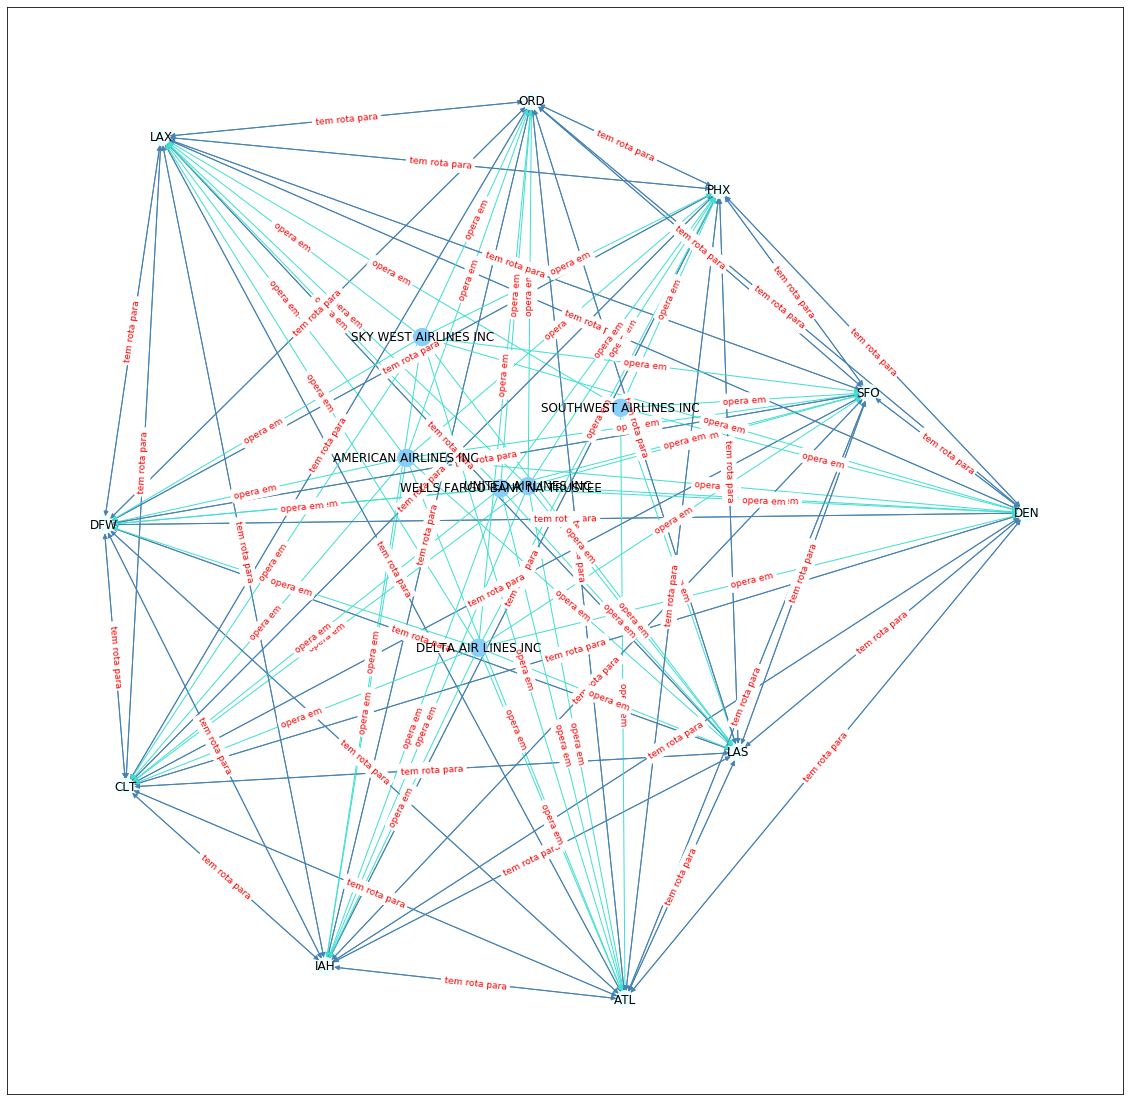
\includegraphics[width = \textwidth]{Imagens/preview.png}
    \caption{Grafo mais limpo das companhias e rotas}
    \label{preview}
\end{figure}

Feitas tais modificações, a eficiência do código estava abaixo do satisfatório\footnote{Algumas vezes demorava cerca de 30 segundos para gerar um grafo!}, dessa forma incluímos uma nova restrição, mas dessa vez no banco, onde passamos a considerar apenas os dados de maio de 2020\footnote{A opção por criar um novo banco e não fazer a restrição via query se deu pelo fato do banco completo ter na ordem de 10 milhões de registros de voos, assim a eficiência do código poderia ser comprometida.}. Além disso, cruzamos os dados de fabricantes com as companhias também, fazendo uma visualização de que fabricantes de aeronave fabricam para cada companhia. No final criamos um grafo interativo onde, onde o usuário pode escolher quantas companhias, aeroportos e fabricantes deseja plotar, limitados a 12, 30 e 5, respectivamente. Os grafos finais poderão ser vistos na próxima seção.

Por fim, vale a pena relatar um problema que ocorreu durante a execução de uma query no Ubuntu. Uma das configurações padrão do MySQL Server estava gerando um erro no \codeword{GROUP BY}. Para resolver esse problema foi adicionada uma linha com o texto \codeword{sql_mode = ""} no final do arquivo localizado em \codeword{/etc/mysql/mysql.conf.d/mysqld.cnf}.

\section{Resultados}

Nos grafos plotados, temos em ``azure'' os aeroportos, em ``lightskyblue'' as companhias e em ``turquoise'' as empresas fabricantes de aeronaves. Conforme a seção anterior, a interação entre aeroportos se dá através de uma aresta que significa que existe uma rota entre dois aeroportos. Já a interação entre companhias e aeroportos se dá por uma arestas que representa que a companhia opera naquele aeroporto e a interação entre companhias e fabricantes se dá por uma aresta que representa que um fabricante fabricou aeronaves para aquela companhia.

Nas Figuras \ref{view1}, \ref{view2}, \ref{view3}, \ref{view4} e \ref{view5} temos algumas das principais visualizações geradas pelo código elaborado. Temos combinações que trazem as três informações como um todo. Também, há grafos com quantidade de aeroportos ou de fabricantes iguais a 0, o que possibilita fazer análises de quem fabrica aeronaves para cada companhia ou que companhia opera em que aeroporto.

Mais visualizações podem ser obtidas diretamente no \href{https://github.com/IgorMichels/USA_Flights_Graphs/blob/main/Grafo\%20-\%20Final.ipynb}{\textbf{painel interativo em Jupyter Notebook}} gerado, o qual está disponível no GitHub \cite{github2} e permite personalização dos três parâmetros utilizados.

\begin{figure}[H]
    \centering
    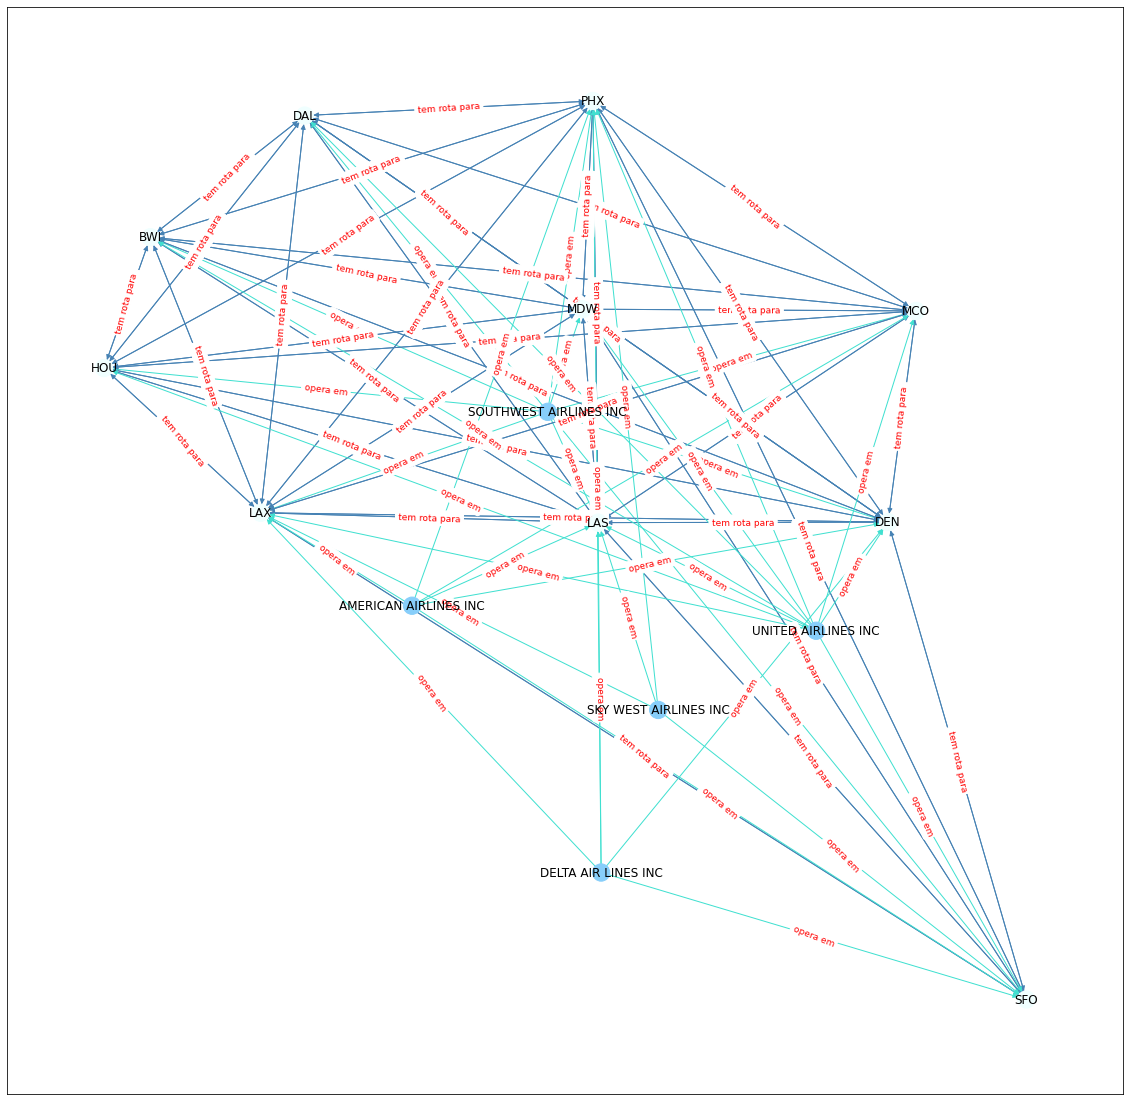
\includegraphics[width = \textwidth]{Imagens/5-10-0.png}
    \caption{5 maiores companhias e os 10 maiores aeroportos, sem fabricantes.}
    \label{view1}
\end{figure}

\begin{figure}[H]
    \centering
    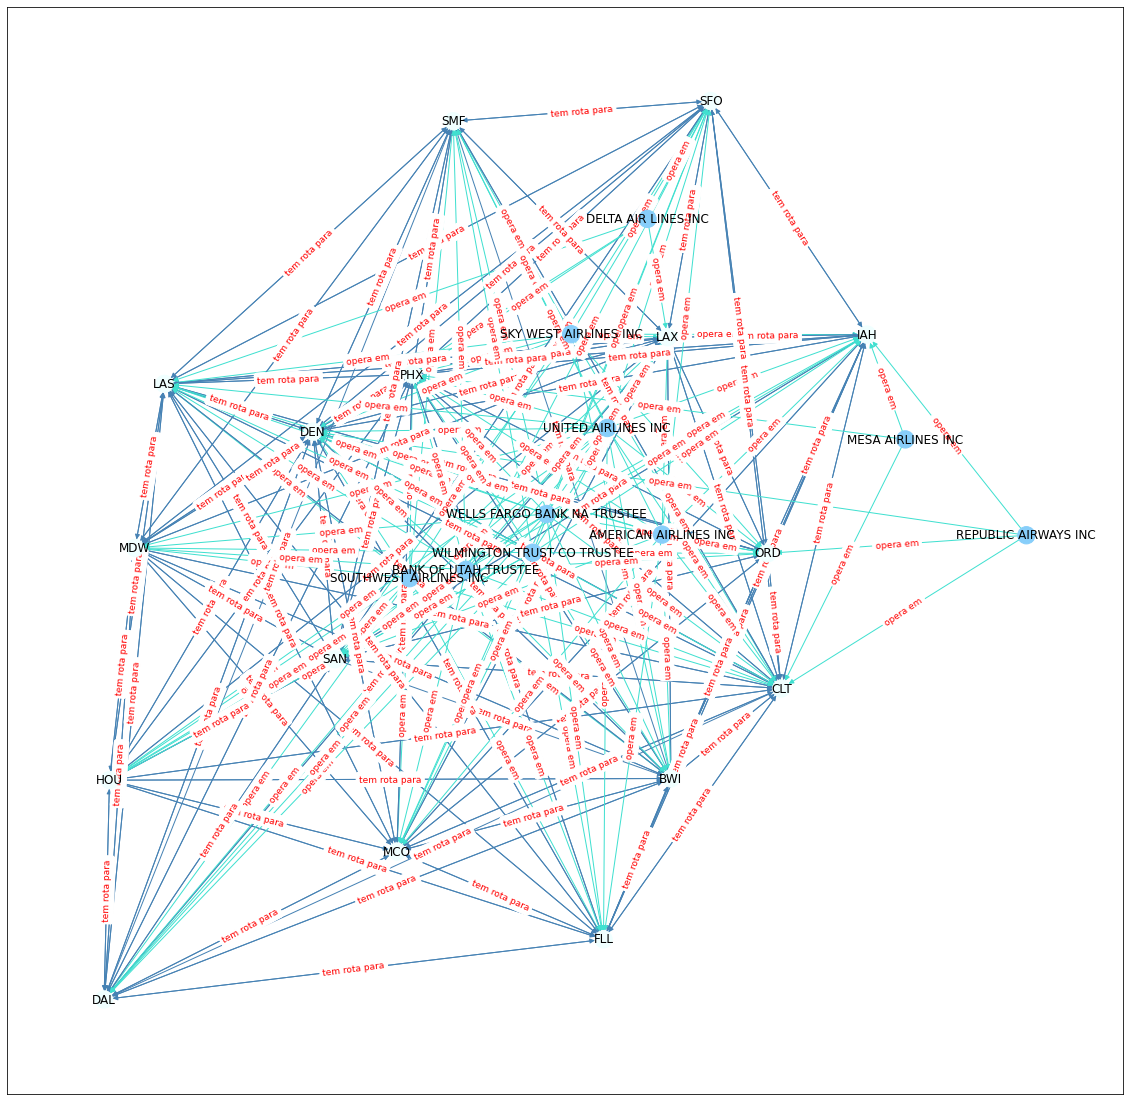
\includegraphics[width = \textwidth]{Imagens/10-16-0.png}
    \caption{10 maiores companhias e os 16 maiores aeroportos, sem fabricantes.}
    \label{view2}
\end{figure}

\begin{figure}[H]
    \centering
    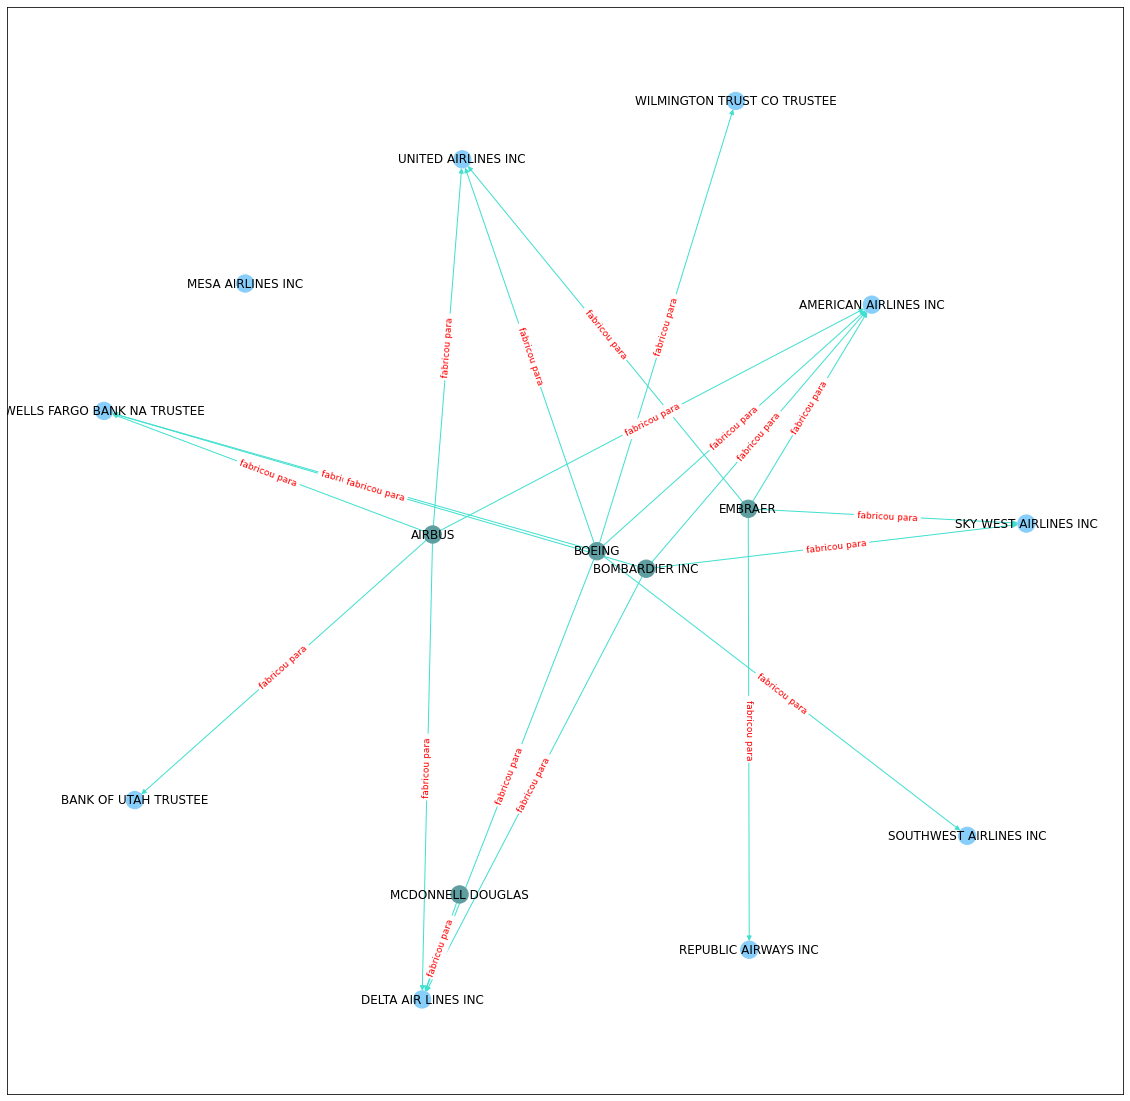
\includegraphics[width = \textwidth]{Imagens/10-0-5.png}
    \caption{10 maiores companhias e os 5 maiores fabricantes, sem aeroportos.}
    \label{view3}
\end{figure}

\begin{figure}[H]
    \centering
    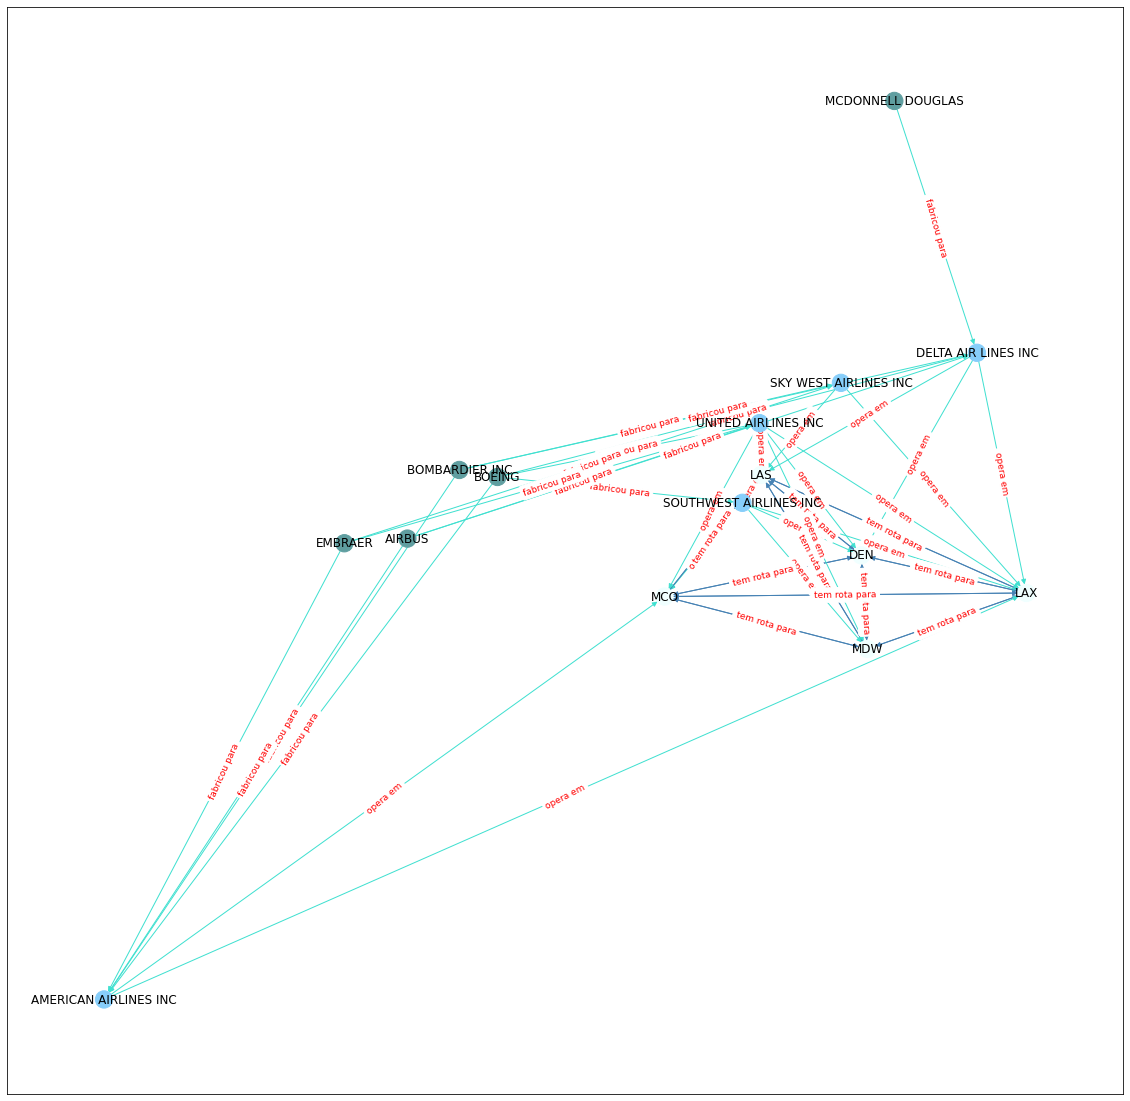
\includegraphics[width = \textwidth]{Imagens/5-5-5.png}
    \caption{5 maiores companhias, os 5 maiores aeroportos e os 5 maiores fabricantes.}
    \label{view4}
\end{figure}

\begin{figure}[H]
    \centering
    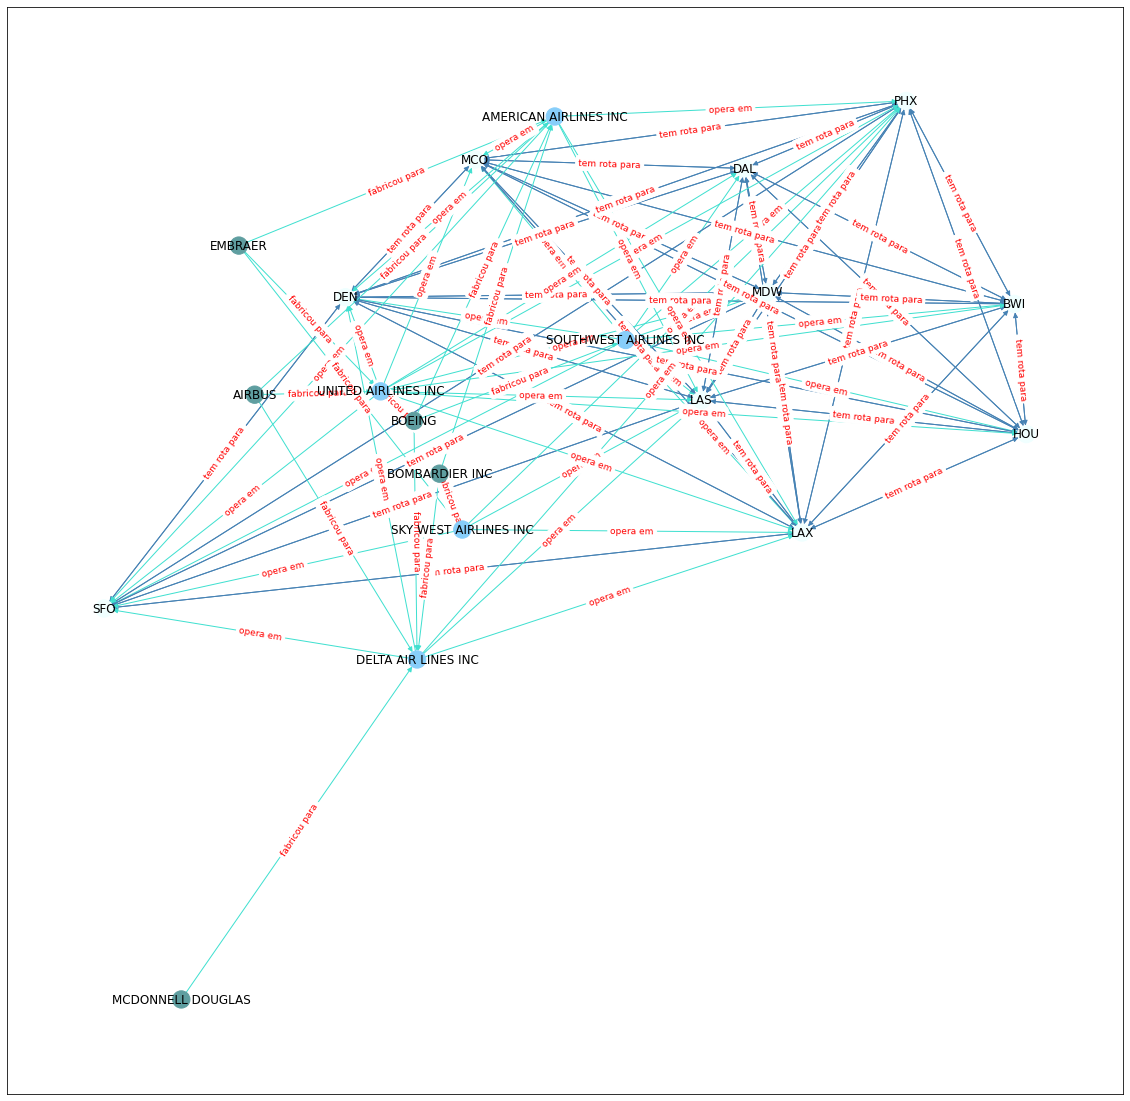
\includegraphics[width = \textwidth]{Imagens/5-10-5.png}
    \caption{5 maiores companhias, os 10 maiores aeroportos e os 5 maiores fabricantes.}
    \label{view5}
\end{figure}

\printbibliography

\end{document}
